\section{Teilversuch 5: Phänomenologische Beobachtung der zirkularen Polarisation (longitudinale Beobachtung)}
	\begin{figure}[!ht]
	    \centering
	   	\begin{subfigure}{0.48\textwidth}
			\centering
			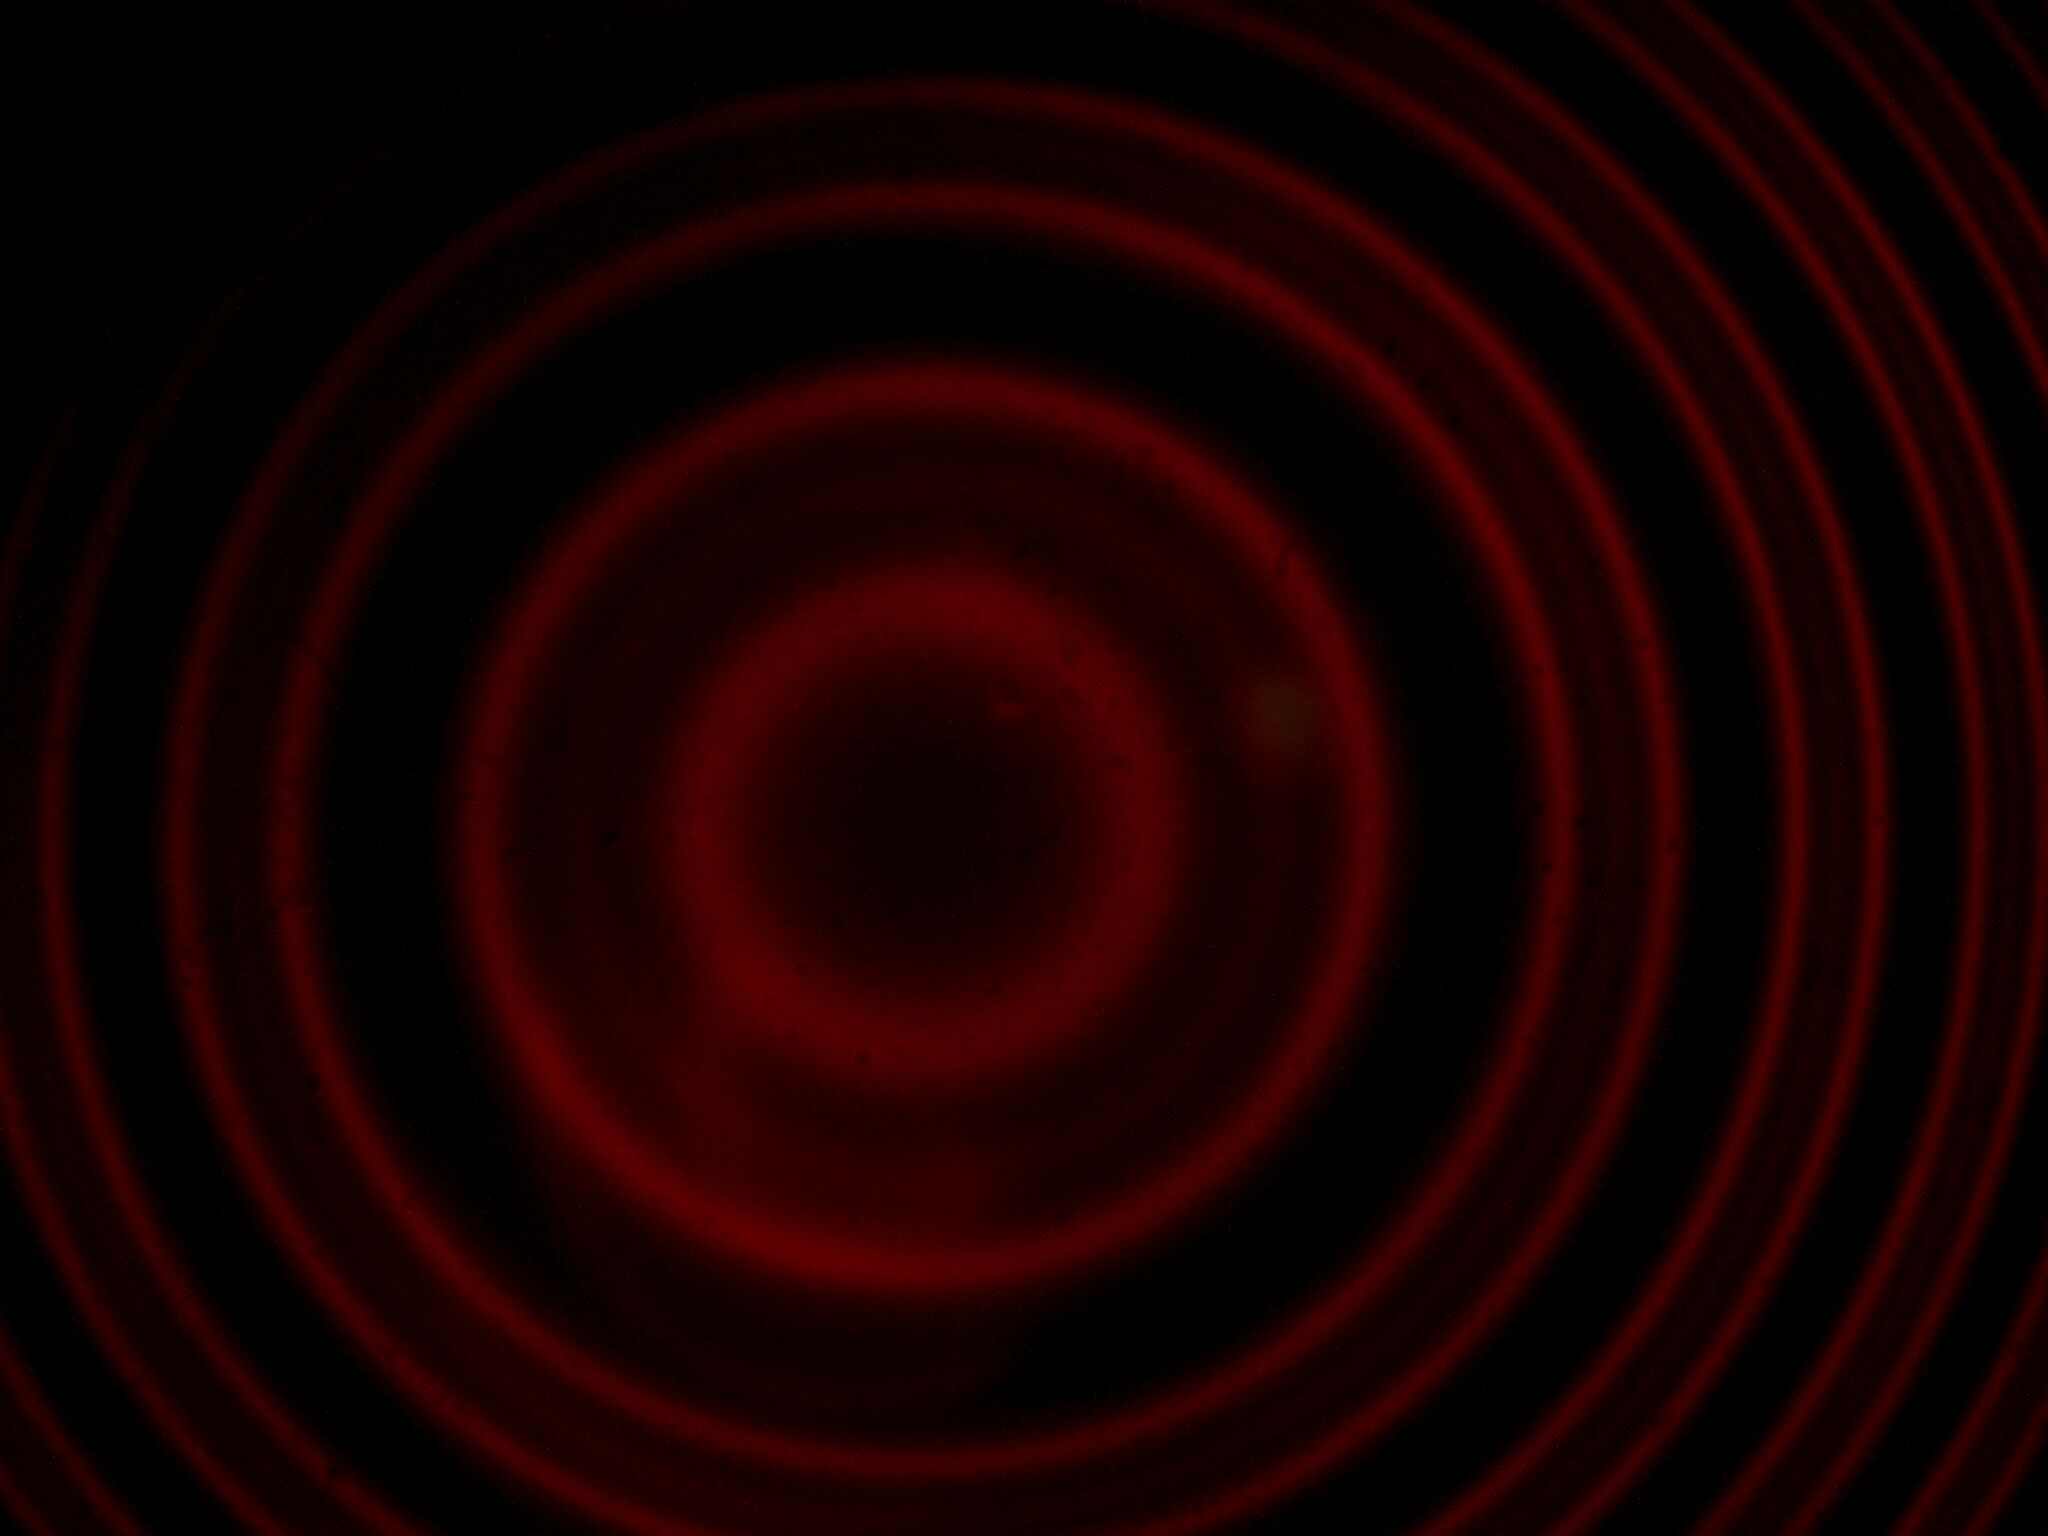
\includegraphics[width=\textwidth]{images/Capture_825.bmp.jpg}
			\caption{$I = \SI{7.31(1)}{\ampere}$}
			\vspace{0.5\baselineskip}
		\end{subfigure}
		\hfill
		\begin{subfigure}{0.48\textwidth}
			\centering
			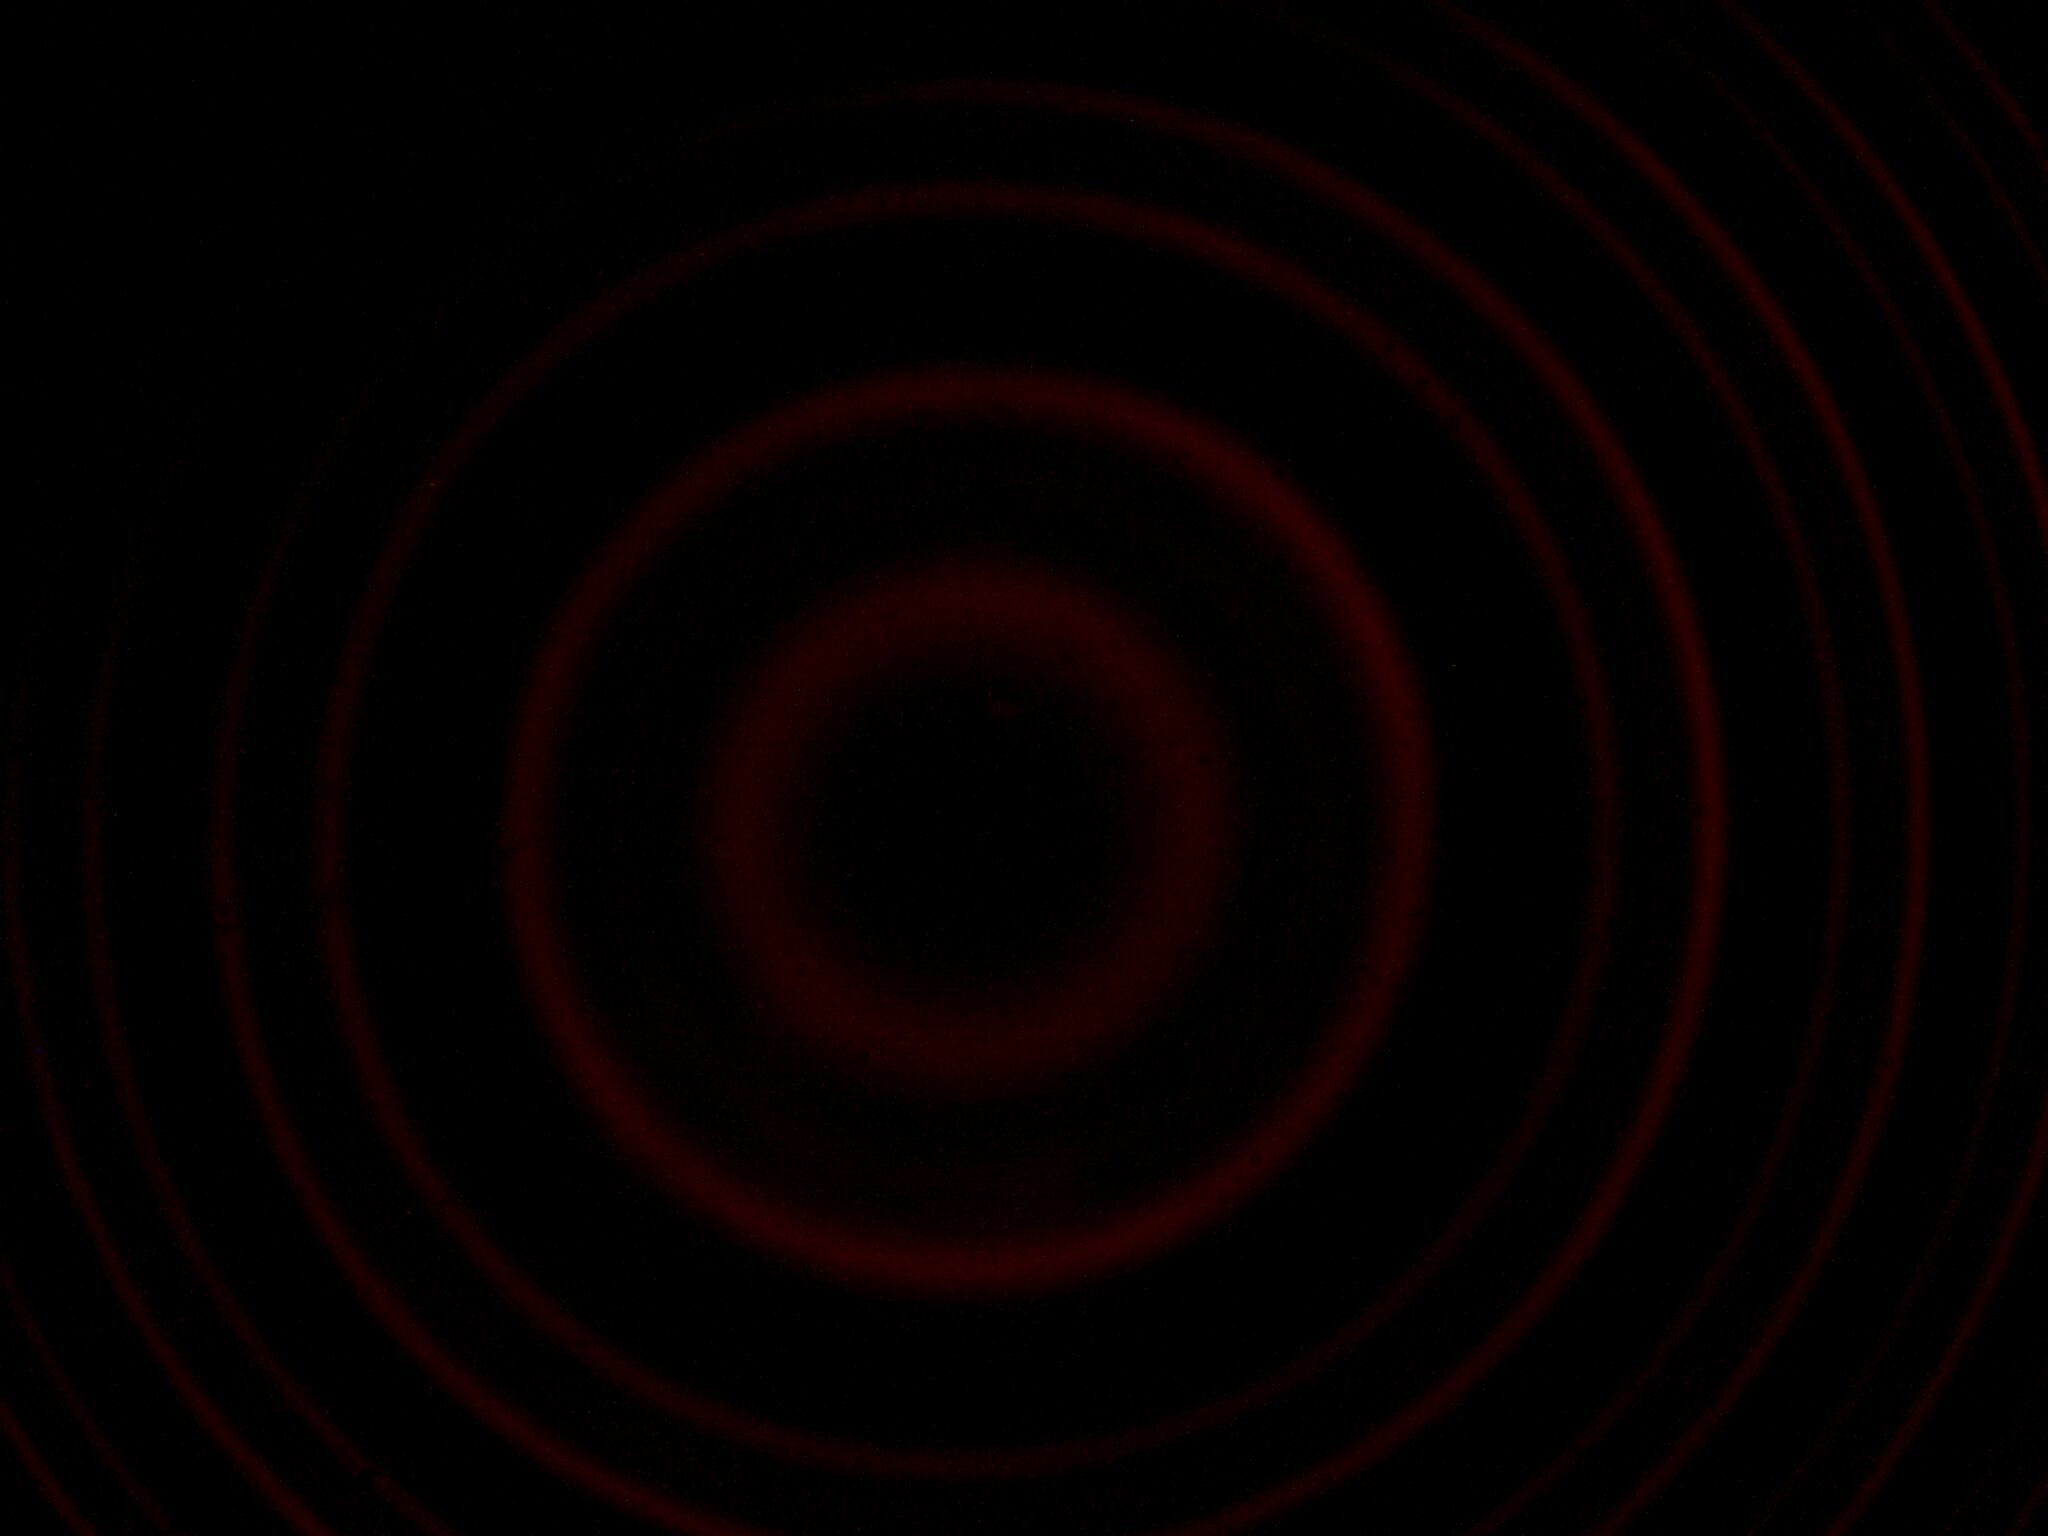
\includegraphics[width=\textwidth]{images/Capture_826.bmp.jpg}
			\caption{Beide Linien sichtbar (Polarisationsfilter eingesetzt)}
			\vspace{0.5\baselineskip}
		\end{subfigure}
		\begin{subfigure}{0.48\textwidth}
			\centering
			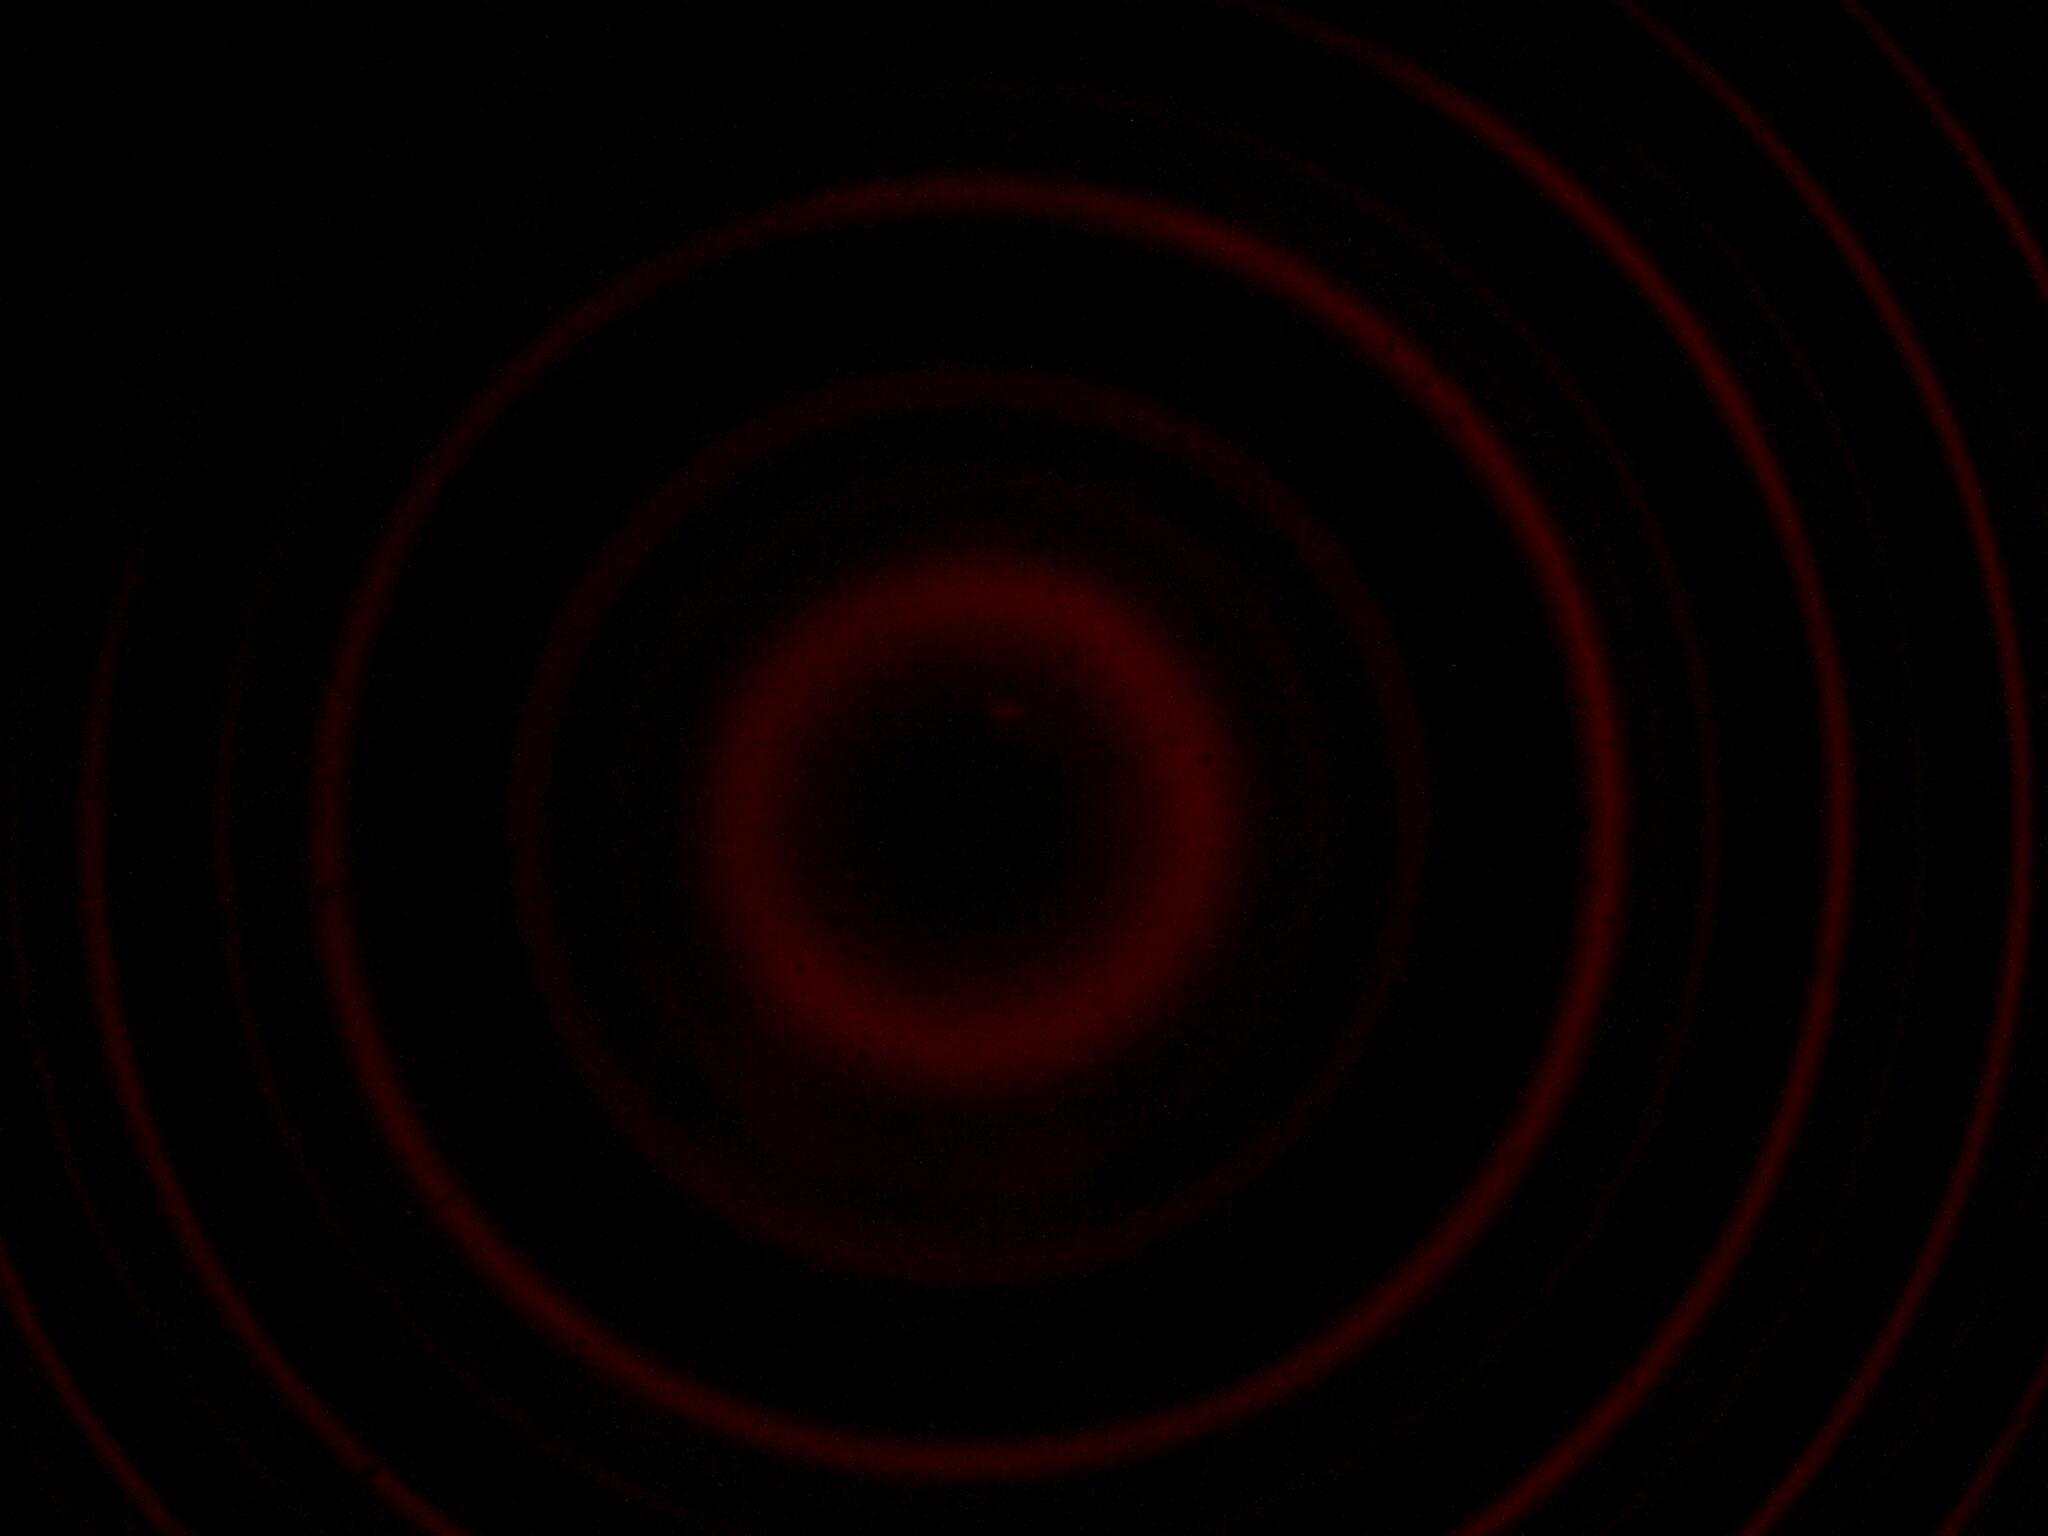
\includegraphics[width=\textwidth]{images/Capture_827.bmp.jpg}
			\caption{$+\SI{45}{\degree}$ Nur innere Ring sichbar}
			\vspace{0.5\baselineskip}
		\end{subfigure}
		\hfill
		\begin{subfigure}{0.48\textwidth}
			\centering
			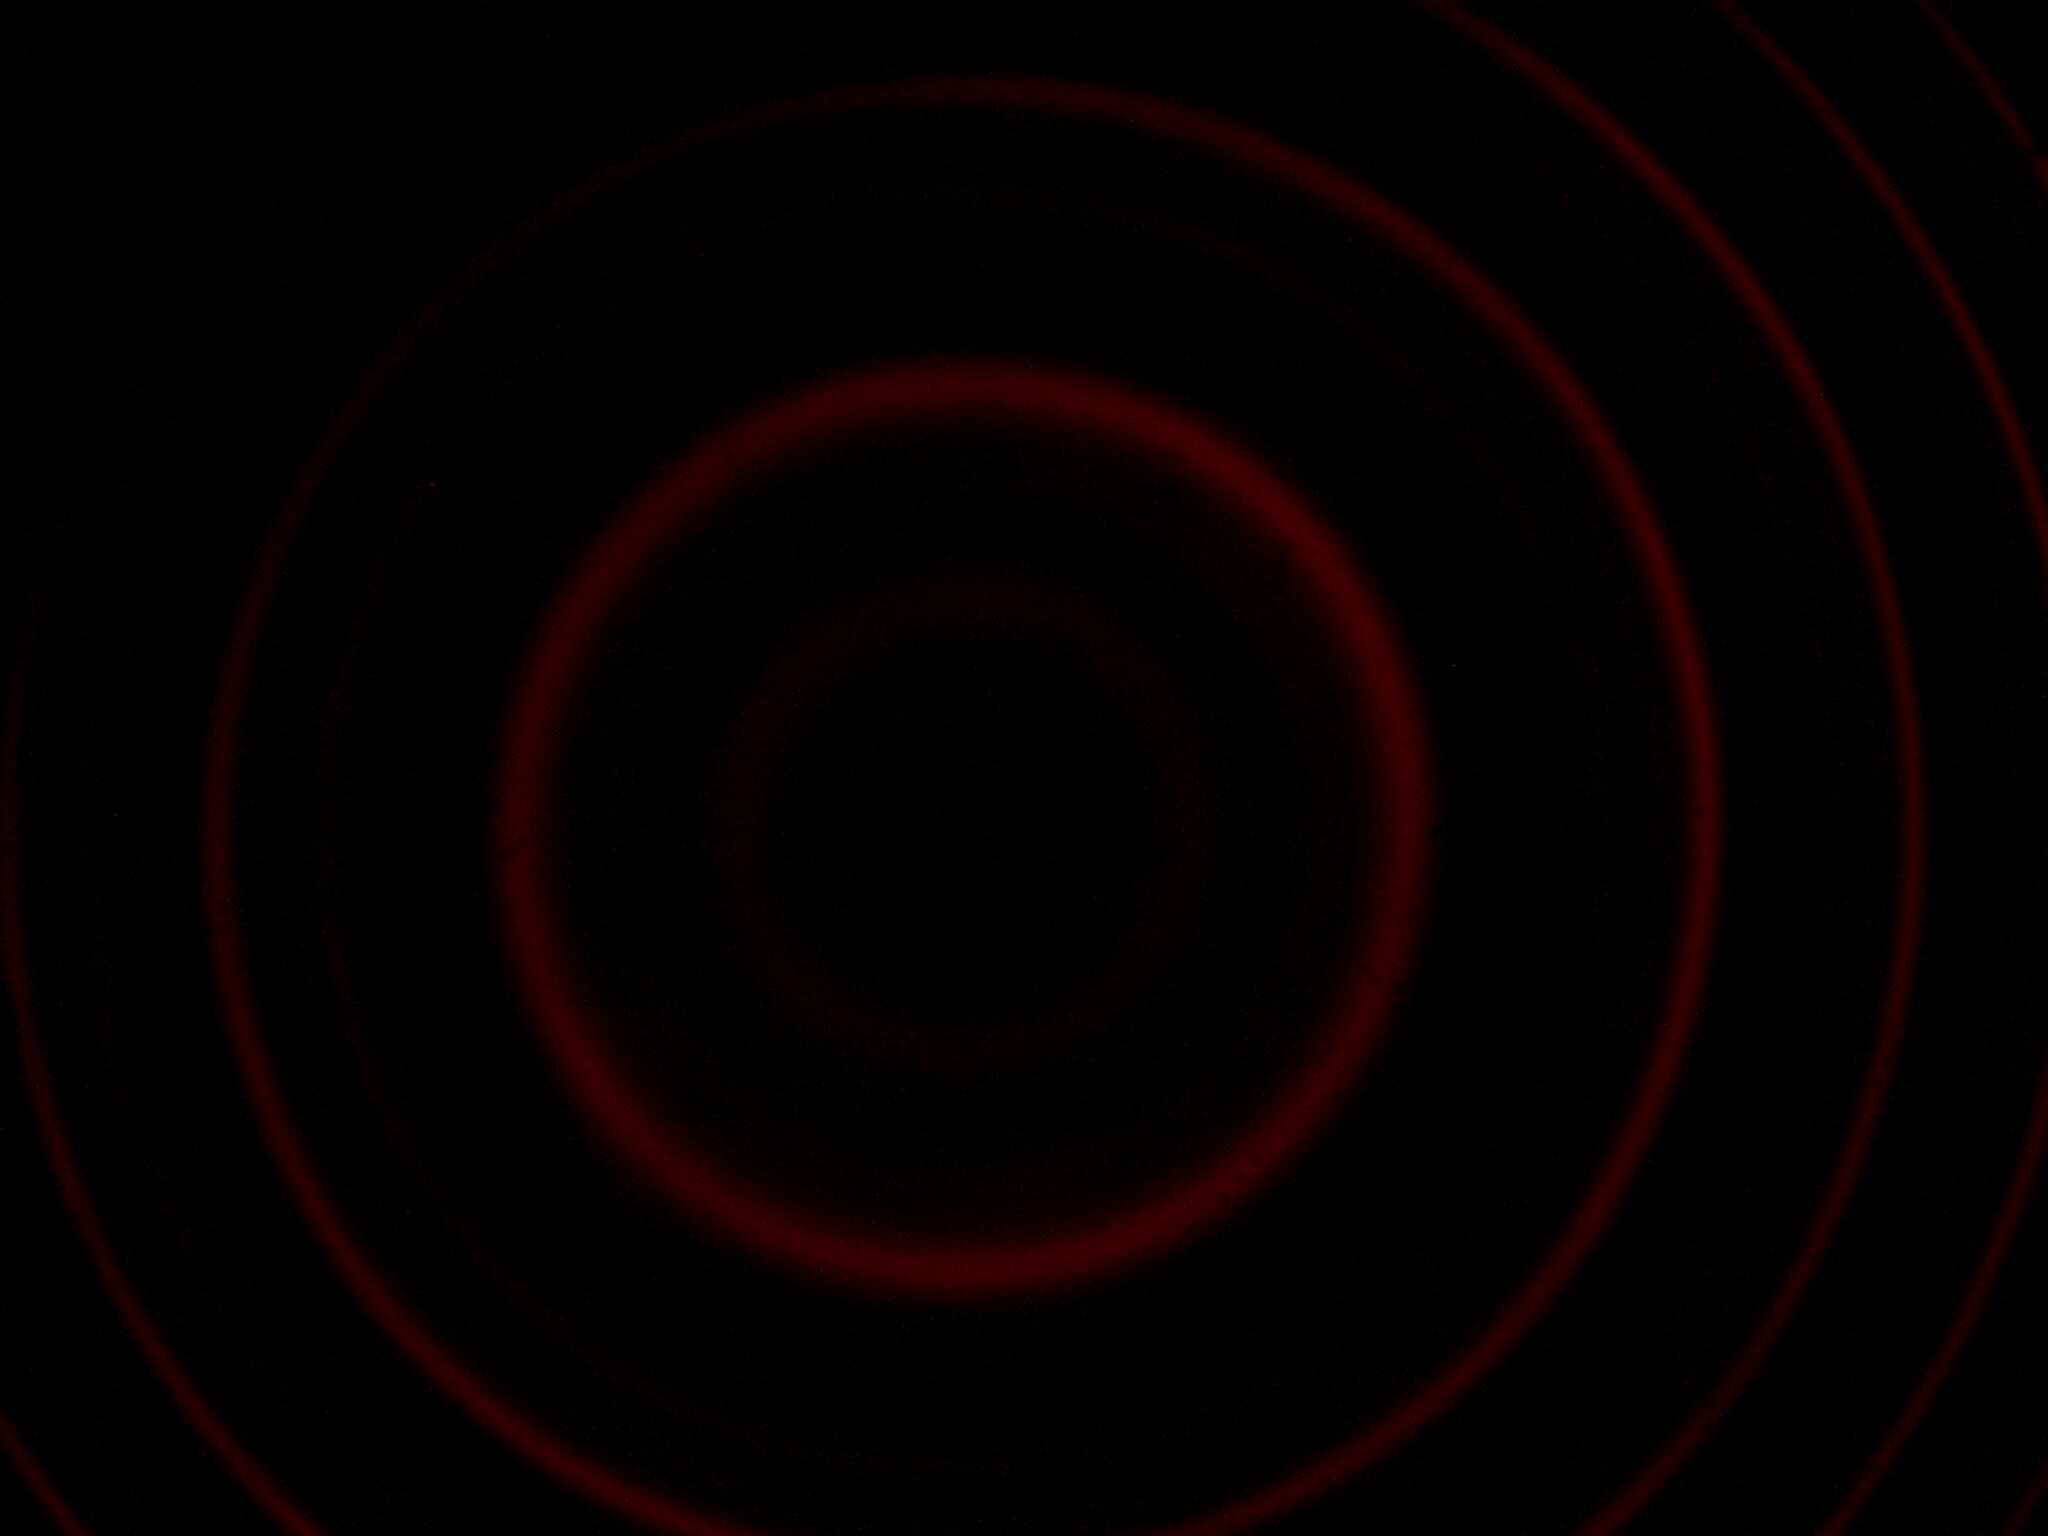
\includegraphics[width=\textwidth]{images/Capture_828.bmp.jpg}
			\caption{$-\SI{45}{\degree}$ Nur äußere Ring sichbar}
			\vspace{0.5\baselineskip}
		\end{subfigure}
	    \caption{Teilversuch 5}
	\end{figure}